\let\negmedspace\undefined
\let\negthickspace\undefined
\documentclass[journal]{IEEEtran}
\usepackage[a5paper, margin=10mm, onecolumn]{geometry}
%\usepackage{lmodern} % Ensure lmodern is loaded for pdflatex
\usepackage{tfrupee} % Include tfrupee package

\setlength{\headheight}{1cm} % Set the height of the header box
\setlength{\headsep}{0mm}     % Set the distance between the header box and the top of the text

\usepackage{gvv-book}
\usepackage{gvv}
\usepackage{cite}
\usepackage{amsmath,amssymb,amsfonts,amsthm}
\usepackage{algorithmic}
\usepackage{graphicx}
\usepackage{textcomp}
\usepackage{xcolor}
\usepackage{txfonts}
\usepackage{listings}
\usepackage{enumitem}
\usepackage{mathtools}
\usepackage{gensymb}
\usepackage{comment}
\usepackage[breaklinks=true]{hyperref}
\usepackage{tkz-euclide} 
\usepackage{listings}
% \usepackage{gvv}                                        
\def\inputGnumericTable{}                                 
\usepackage[latin1]{inputenc}                                
\usepackage{color}                                            
\usepackage{array}                                            
\usepackage{longtable}                                       
\usepackage{calc}                                             
\usepackage{multirow} 
\usepackage{hhline}                                           
\usepackage{ifthen}                                           
\usepackage{lscape}
\usepackage{circuitikz}
\tikzstyle{block} = [rectangle, draw, fill=blue!20, 
    text width=4em, text centered, rounded corners, minimum height=3em]
\tikzstyle{sum} = [draw, fill=blue!10, circle, minimum size=1cm, node distance=1.5cm]
\tikzstyle{input} = [coordinate]
\tikzstyle{output} = [coordinate]

\begin{document}
\bibliographystyle{IEEEtran}
\vspace{3cm}

\title{MatGeo Assignment 4.13.76}
\author{AI25BTECH11007}
 \maketitle
% \newpage
% \bigskip
{\let\newpage\relax\maketitle}

\renewcommand{\thefigure}{\theenumi}
\renewcommand{\thetable}{\theenumi}
\setlength{\intextsep}{10pt} % Space between text and floats


\numberwithin{equation}{enumi}
\numberwithin{figure}{enumi}
\renewcommand{\thetable}{\theenumi}
\noindent
\textbf{Question:}\\
 Two lines

\[
L_1 : \frac{x}{5} \;=\; \frac{y}{3-\alpha} \;=\; \frac{z}{-2}
\]

\[
L_2 : \frac{x}{\alpha} \;=\; \frac{y}{-1} \;=\; \frac{z}{2-\alpha}
\]

are coplanar. Then the value(s) of \(\alpha\)

\textbf{Solution:}\\
\[
L_1 : \frac{x}{5}=\frac{y}{3-\alpha}=\frac{z}{-2},\qquad
L_2 : \frac{x}{\alpha}=\frac{y}{-1}=\frac{z}{2-\alpha}.
\]

\[
\text {Direction vectors are :   } 
\mathbf n_1=\myvec{5\\[2pt]3-\alpha\\[2pt]-2},\qquad
\mathbf n_2=\myvec{\alpha\\[2pt]-1\\[2pt]2-\alpha}.
\]

\[
\text{Choose points on each line, as both lines pass through the origin, so, }\\
\mathbf p_1=\mathbf p_2=\myvec{0\\0\\0}.
\]

Two lines are coplanar iff
\[
\operatorname{rank}\big(\, \myvec{\mathbf n_1 & \mathbf n_2 & \mathbf p_2-\mathbf p_1}\,\big)\le 2.
\]
Here \(\mathbf p_2-\mathbf p_1=\myvec{0\\0\\0}\), so the matrix becomes
\[
\myvec{5 & \alpha & 0\\[2pt] 3-\alpha & -1 & 0\\[2pt] -2 & 2-\alpha & 0},
\]
whose rank is at most \(2\) for every \(\alpha\). Hence the two lines are coplanar for all real \(\alpha\).

\[
\boxed{\alpha\in\mathbb R}
\]

\begin{figure}[H]
    \centering
    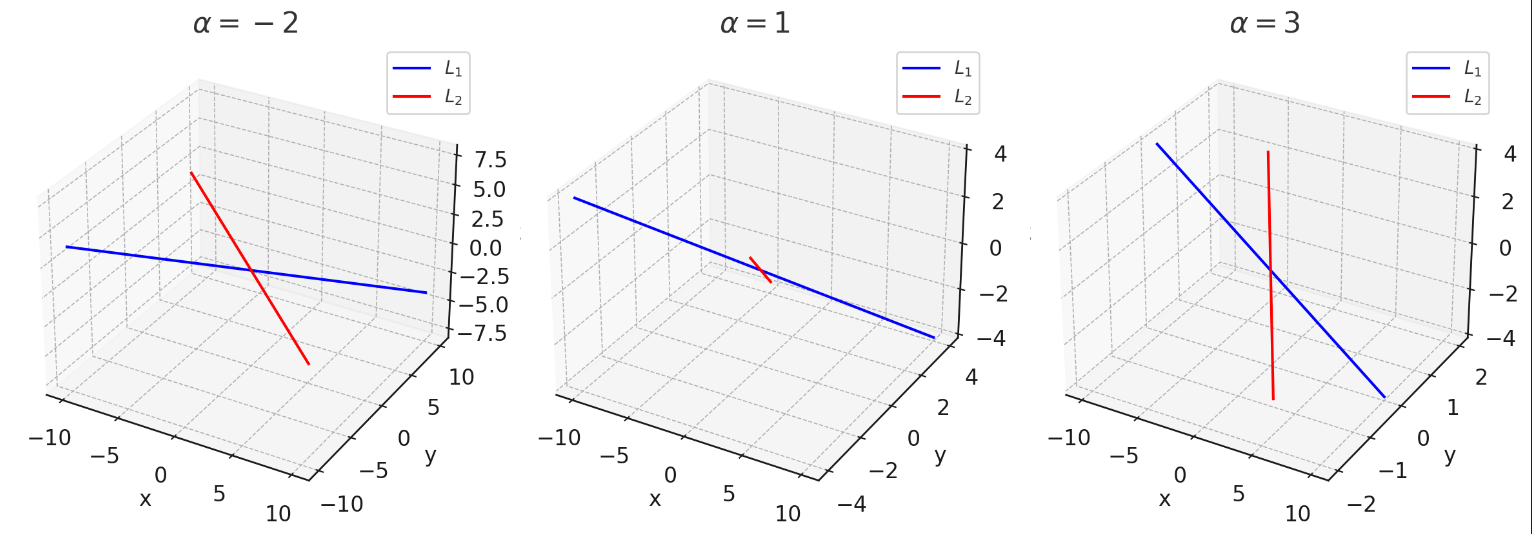
\includegraphics[width=1.0\linewidth]{figs/image.png}
    \caption{Image}
    \label{fig:placeholder}
\end{figure}
\end{document}
